% Pedigree showing the relationship types: siblings, half-siblings, step-siblings, 1st cousins,
% co-cousins. Standalone; built by poster/build.sh into pedigree.pdf and included in the poster.
% Solid connectors = biological relatives; dashed = relatives-in-law (no shared ancestry).
\documentclass[tikz, border=4mm]{standalone}
\usepackage[T1]{fontenc}
\usepackage{lmodern}
\usepackage[default]{sourcesans}
\usetikzlibrary{positioning, calc}

% Okabe-Ito (colour-blind safe)
\definecolor{cSib}{HTML}{0072B2}
\definecolor{cHalf}{HTML}{009E73}
\definecolor{cStep}{HTML}{D55E00}
\definecolor{cCous}{HTML}{CC79A7}
\definecolor{cCoc}{HTML}{E69F00}
\definecolor{ink}{HTML}{1F2328}
\definecolor{founder}{HTML}{FFFFFF}
\definecolor{proband}{HTML}{DDE3EA}

\tikzset{
  ped/.style={draw=ink, line width=1.2pt},
  male/.style={ped, rectangle, minimum size=7.5mm, inner sep=0pt, fill=#1},
  female/.style={ped, circle, minimum size=8.2mm, inner sep=0pt, fill=#1},
  male/.default=founder, female/.default=founder,
  mate/.style={ped},
  descent/.style={ped},
  lab/.style={font=\small, text=ink},
  rel/.style={line width=3.2pt, rounded corners=6pt, line cap=round},
  inlaw/.style={dash pattern=on 7pt off 4pt},
  rellab/.style={font=\small\bfseries, fill=white, inner sep=1.5pt},
}

% (x, y) layout: generation rows at y = 0, -2.6, -5.2 (cm)
\newcommand{\gA}{0}
\newcommand{\gB}{-2.6}
\newcommand{\gC}{-5.2}

\begin{document}
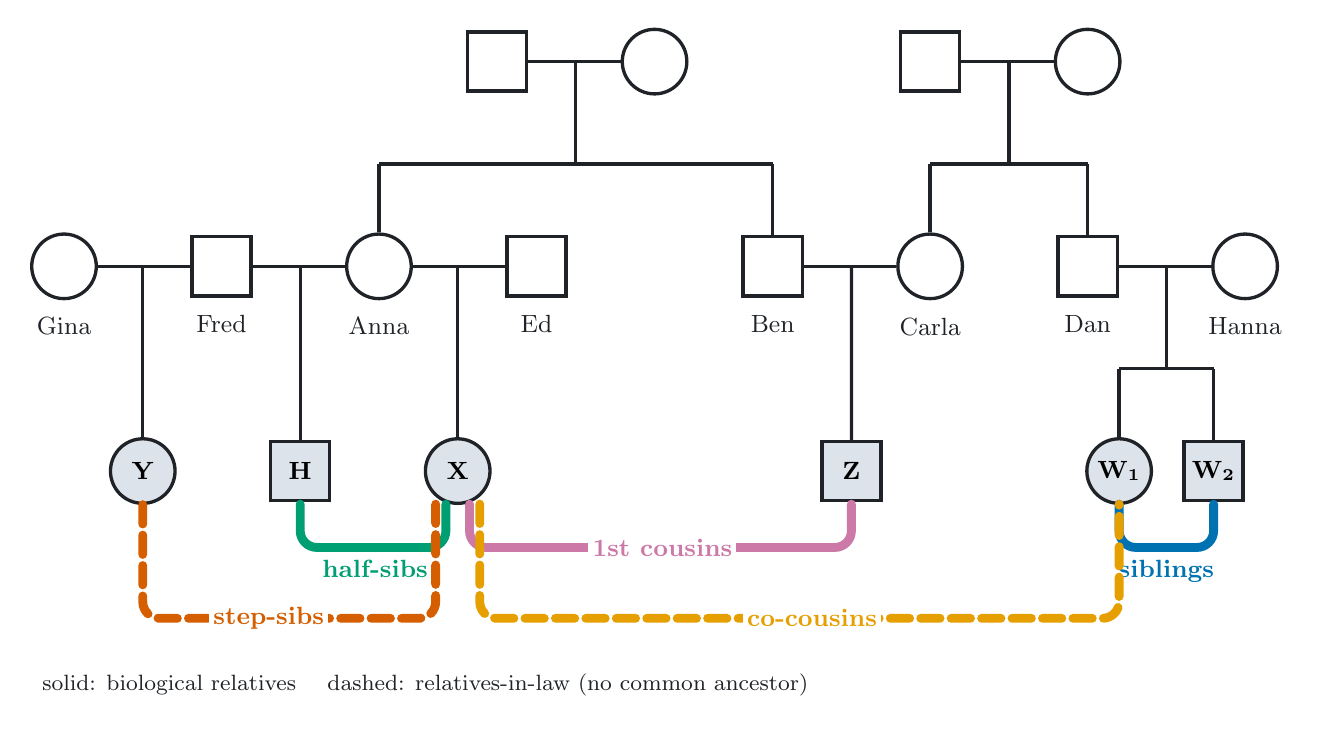
\begin{tikzpicture}[x=1cm, y=1cm]

% ---------------- generation 1: two sets of grandparents ----------------
\node[male]   (g1m) at (5.5,\gA) {};
\node[female] (g1f) at (7.5,\gA) {};
\node[male]   (g2m) at (11,\gA) {};
\node[female] (g2f) at (13,\gA) {};
\draw[mate] (g1m) -- (g1f);
\draw[mate] (g2m) -- (g2f);

% ---------------- generation 2 ----------------
\node[female] (gina)  at (0,\gB)  {};  \node[lab, below=1mm of gina]  {Gina};
\node[male]   (fred)  at (2,\gB)  {};  \node[lab, below=1mm of fred]  {Fred};
\node[female] (anna)  at (4,\gB)  {};  \node[lab, below=1mm of anna]  {Anna};
\node[male]   (ed)    at (6,\gB)  {};  \node[lab, below=1mm of ed]    {Ed};
\node[male]   (ben)   at (9,\gB)  {};  \node[lab, below=1mm of ben]   {Ben};
\node[female] (carla) at (11,\gB) {};  \node[lab, below=1mm of carla] {Carla};
\node[male]   (dan)   at (13,\gB) {};  \node[lab, below=1mm of dan]   {Dan};
\node[female] (hanna) at (15,\gB) {};  \node[lab, below=1mm of hanna] {Hanna};

% sibships of generation 2
\draw[descent] ($(g1m)!0.5!(g1f)$) -- ++(0,-1.3) coordinate (s1);
\draw[descent] (4,\gB+1.3) -- (9,\gB+1.3);
\draw[descent] (anna.north) -- (4,\gB+1.3);
\draw[descent] (ben.north)  -- (9,\gB+1.3);
\draw[descent] ($(g2m)!0.5!(g2f)$) -- ++(0,-1.3);
\draw[descent] (11,\gB+1.3) -- (13,\gB+1.3);
\draw[descent] (carla.north) -- (11,\gB+1.3);
\draw[descent] (dan.north)   -- (13,\gB+1.3);

% matings of generation 2 (Fred and Anna each have two partners)
\draw[mate] (gina) -- (fred);
\draw[mate] (fred) -- (anna);
\draw[mate] (anna) -- (ed);
\draw[mate] (ben) -- (carla);
\draw[mate] (dan) -- (hanna);

% ---------------- generation 3 (the relatives compared) ----------------
\node[female=proband, font=\small\bfseries] (y)  at (1,\gC)    {Y};
\node[male=proband,   font=\small\bfseries] (h)  at (3,\gC)    {H};
\node[female=proband, font=\small\bfseries] (x)  at (5,\gC)    {X};
\node[male=proband,   font=\small\bfseries] (z)  at (10,\gC)   {Z};
\node[female=proband, font=\small\bfseries] (w1) at (13.4,\gC) {W\textsubscript{1}};
\node[male=proband,   font=\small\bfseries] (w2) at (14.6,\gC) {W\textsubscript{2}};

\foreach \a/\b/\c in {gina/fred/y, fred/anna/h, anna/ed/x, ben/carla/z} {
  \draw[descent] ($(\a)!0.5!(\b)$) -- (\c.north);
}
\draw[descent] ($(dan)!0.5!(hanna)$) -- ++(0,-1.3) coordinate (s3);
\draw[descent] (13.4,\gC+1.3) -- (14.6,\gC+1.3);
\draw[descent] (w1.north) -- (13.4,\gC+1.3);
\draw[descent] (w2.north) -- (14.6,\gC+1.3);

% ---------------- relationship connectors (below generation 3) ----------------
% each: down from proband A, across, up to proband B; depth staggers the connectors
\def\base{\gC-0.42}
% siblings: W1 - W2
\draw[rel, cSib]  (13.4,\base) -- (13.4,\base-0.55) -- (14.6,\base-0.55) -- (14.6,\base);
\node[rellab, text=cSib, below=1mm] at (14.0,\base-0.55) {siblings};
% half-siblings: X - H (share mother Anna)
\draw[rel, cHalf] (4.85,\base) -- (4.85,\base-0.55) -- (3,\base-0.55) -- (3,\base);
\node[rellab, text=cHalf, below=1mm] at (3.95,\base-0.55) {half-sibs};
% step-siblings: X - Y (X's mother had a child with Y's father)
\draw[rel, cStep, inlaw] (4.72,\base) -- (4.72,\base-1.45) -- (1,\base-1.45) -- (1,\base);
\node[rellab, text=cStep] at (2.6,\base-1.45) {step-sibs};
% 1st cousins: X - Z (mother Anna and father Ben are siblings)
\draw[rel, cCous] (5.15,\base) -- (5.15,\base-0.55) -- (10,\base-0.55) -- (10,\base);
\node[rellab, text=cCous] at (7.6,\base-0.55) {1st cousins};
% co-cousins: X - W1 (X's uncle Ben married W1's aunt Carla; they share cousin Z)
\draw[rel, cCoc, inlaw] (5.28,\base) -- (5.28,\base-1.45) -- (13.4,\base-1.45) -- (13.4,\base);
\node[rellab, text=cCoc] at (9.5,\base-1.45) {co-cousins};

% key
\node[lab, anchor=west, font=\footnotesize] at (-0.4,\base-2.3)
  {solid: biological relatives \quad dashed: relatives-in-law (no common ancestor)};

\end{tikzpicture}
\end{document}
